\section{实验1:AI与人类专家在不同人格特质广告生成中的比较} 

\label{实验1:GPT-4与人类专家在不同人格特质广告生成中的比较}

\subsection{方法}
本实验采用 \textbf{2(信息创作者:AI/人类专家)}的被试间设计。AI条件选取当前表现最优的模型GPT-4,人类专家以心理学专业研究生作为代表。广告通过针对五种不同人格水平(外倾性、开放性、尽责性、宜人性、神经质)的高水平特质进行个性化设计,即分别为高外倾、高开放、高尽责、高宜人和高神经质的消费者设计了广告内容。每类信息创作者(AI/人类专家)针对每种人格水平生成 3-5 则广告,每位被试被随机分配到一类信息创作者的广告条件,并从每个人格水平对应的 3 则广告中随机选择 1 则进行呈现。被试依次观看五则广告(对应五种人格水平),广告呈现顺序随机,且需对每则广告进行评价。

\textbf{(1)被试}

通过见数平台发布实验,366名参与者自愿参加这项研究。28名参与者由于注意检查测试未通过被剔除,剩余\textbf{322}名有效被试(年龄范围= 18-58岁;\textit{M}=29.43岁;\textit{SD}=7.36;女性203名)。参与任务的每名参与者获得5元人民币作为报酬。其中注意力检测题为一道见数平台自带的题目:“今天天气不错,请选2”,若未选2,则被判定为注意力检测题未通过。

\textbf{(2)问卷测量}

a. 大五人格量表。BFI10量表(详见同研究一实验1 \ref{study1-substudy1-measurement})。

b. 说服效果。具体的题项与实验1一致(详见 \ref{study1-substudy1-measurement},包含五个题项,用于评估参与者对广告和产品的态度以及购买意图。每个题项均采用1-5点李克特量表评分,广告说服效果的总评分为五个题项得分的平均值。

\textbf{(3)广告材料}

针对2(信息创作者:AI/人类专家)*5(广告人格:外倾性/开放性/尽责性/宜人性/神经质)共10个条件生成广告材料。AI条件选取当前表现最优的模型GPT,人类专家以心理学专业研究生作为代表。根据前人文献选择中性的产品手机,广告描述避免具体品牌名以排除品牌的影响。提供给GPT和人类专家的指导语是相同的,包括对目标消费者特点的描述(个性化,具体的人格描述参考人格特质量表中的描述)以及广告基本特征的描述。

每个条件生成5-6个信息,初始生成53则广告文本材料,经过预实验筛选,剩余38条(详见附录)。通过见数平台发布实验,140名参与者自愿参加预实验(年龄范围= 18-65岁;\textit{M}=32.26岁;\textit{SD}=10.05;女性69名)。每名参与者只看一个条件中的随机一则广告文本材料,条件之间的顺序随机。阅读完一则广告文本材料后,参与者需要选择这则广告面向的消费者特点,并对广告理解(消费者能够理解该信息是在宣传手机)/相关程度(该广告与手机这一产品的相关程度)进行1-5点量表的评价。对于消费者特点,参与者需要在五个目标人格特点描述中选择与广告最相符的特点,描述同样参考人格特质量表中对特质的描述。我们通过两个筛选条件来选择用于正式实验的实验材料: 1)广告人格是选择目标人格是最多的;2)理解程度和相关程度均大于3分。最终筛选得到每个条件3-5则广告文本材料,具体的实验材料详见附录。

\subsection{实验流程} 
在实验开始前,参与者被告知接下来他们将对五则社交媒体上的广告进行评价。所有广告文案的配图相同(见图\ref{fig:Study2-exp1-ad-example}),区别在于广告文案内容。参与者将依次阅读五则广告的文案,并在每阅读完一则文案后立即对其说服效果进行评分。完成所有五则广告文案的评价后,参与者需回答与人格测试相关的问卷题目,最后提供年龄、性别等人口统计学信息。

\begin{figure}[htbp]
    \centering
    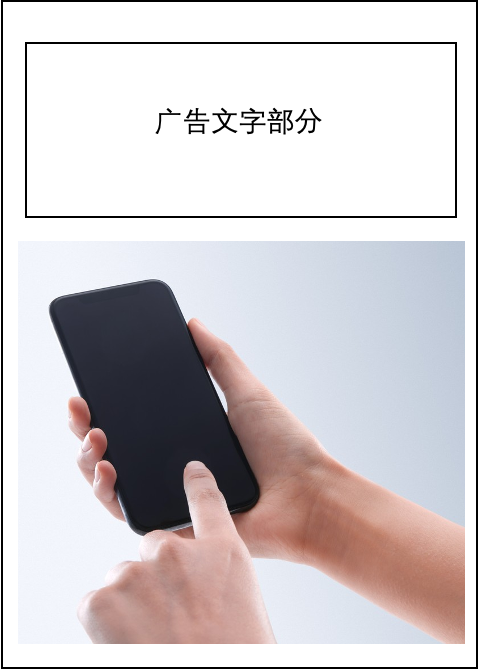
\includegraphics[width=.3\linewidth]{Image/Study2-exp1.png}
    \caption{\label{fig:Study2-exp1-ad-example}实验开始前的广告示意图}
\end{figure}

\subsection{结果}
首先分别对不同创作者(人类专家/GPT-4)生成的个性化广告效果进行检验。个性化效果通过建立人格水平与说服效果之间的线性回归模型来进行衡量,其中人格水平作为自变量,说服效果作为因变量。由于在本研究中,个性化广告是针对各人格维度的高水平个体进行设计的,因此理论上,当参与者在某一人格维度的得分越高时,相应该维度的个性化广告的说服效果越好。回归结果如下表所示(表 \ref{tab:study1_traitResults})。

结果表明,在GPT-4生成的广告中,宜人性(\textit{$\beta$} = 0.3765, \textit{p} = 0.002)、外倾性(\textit{$\beta$} = 0.1967, \textit{p} < 0.001)、尽责性(\textit{$\beta$} = 0.2978, \textit{p} < 0.001)、开放性(\textit{$\beta$} = 0.2808, \textit{p} = 0.001)四个维度上表现出人格水平对说服效果的显著正向预测效果,即宜人性/外倾性/尽责性/开放性水平越高的参与者,针对各维度高水平设计的广告说服效果更好。而神经质表现出显著相反的趋势(\textit{$\beta$} = -0.2479, \textit{p} < 0.001),即神经质水平越低越喜欢针对高神经质设计的广告。

在人类专家生成的广告中,仅宜人性(\textit{$\beta$} = 0.2685, \textit{p} = 0.004)和开放性(\textit{$\beta$} = 0.2399, \textit{p} = 0.016) 两个维度上表现出人格水平对说服效果的显著正向预测效果,即宜人性/开放性水平越高的参与者,针对各维度高水平设计的广告说服效果更好。外倾性维度上正向预测效果达到边缘显著水平(\textit{$\beta$} = 0.1343, \textit{p} = 0.087),尽责性人格水平呈正向预测效果但不显著(\textit{$\beta$} = 0.0932, \textit{p} = 0.229),而神经质人格水平的预测效果呈负向但不显著(\textit{$\beta$} = -0.1176, \textit{p} = 0.12)。

为进一步探讨人类专家与GPT-4在个性化广告创作水平上的差异,本研究对两类创作者回归斜率的差异进行了显著性检验。结果表明仅在尽责性维度上,人类专家与GPT-4的个性化水平之间差异达到边缘显著水平(\textit{t}(318) = 1.8128, \textit{p} = 0.07),具体而言,GPT-4生成的广告在该维度表现出显著的个性化效果,而人类专家的个性化效果不显著;在外倾性维度上,尽管两类信息创作者表现出不一样的趋势,即GPT-4的个性化水平显著,但人类专家的个性化水平边缘显著,但两者之间的斜率差异未达到显著水平(\textit{t}(318) = 0.6486, \textit{p} = 0.52);在宜人性(\textit{t}(318) = 0.7245, \textit{p} = 0.47)和开放性(\textit{t}(318) = 0.3115, \textit{p} = 0.76)维度上,GPT-4和人类专家在生成的个性化广告效果均显著,但两者之间不存在显著差异;在神经质维度,尽管两者存在一定的差异,但仍未达到显著水平(\textit{t}(318) = 1.4269, \textit{p} = 0.15)。

\FloatBarrier % 防止表格与正文之间的分离,强制插入位置

% \begin{table}[H]
%     \centering
%     \caption{\label{tab:study1_traitResults} 人格特质回归分析结果}
%     {\tablesongti % 整个表格环境应用宋体六号字体
%     \renewcommand{\arraystretch}{1} % 调整行距
%     \begin{tabularx}{\linewidth}{>{\raggedright\arraybackslash}X X c c c c c c}
%         \toprule
%         个性化特质 & 信息创作者 & 系数 & 标准误差 & \textit{t} & \textit{P} $>|t|$ & [0.025 & 0.975] \\ 
%         \midrule
%         \textbf{宜人性}   & \textbf{人类专家}  & 0.2685 & 0.0930 & 2.8860\textsuperscript{**} & 0.004   & 0.0848 & 0.4522 \\
%         \textbf{宜人性}   & \textbf{GPT-4}   & 0.3765 & 0.1166 & 3.2296\textsuperscript{**} & 0.002   & 0.1463 & 0.6068 \\
%         外倾性    & 人类专家   & 0.1343 & 0.0781 & 1.7206\textsuperscript{\dag} & 0.087   & -0.0198 & 0.2884 \\
%         \textbf{外倾性}    & \textbf{GPT-4}     & 0.1967 & 0.0562 & 3.5003\textsuperscript{***} & <0.001  & 0.0857 & 0.3077 \\
%         神经质     & 人类专家      & -0.1176 & 0.0752 & -1.5647 & 0.120   & -0.2661 & 0.0308 \\
%         \textbf{神经质}     & \textbf{GPT-4} & -0.2479 & 0.0518 & -4.7842\textsuperscript{***} & <0.001  & -0.3502 & -0.1455 \\
%         尽责性 & 人类专家  & 0.0932 & 0.0771 & 1.2080 & 0.229   & -0.0591 & 0.2455 \\
%         \textbf{尽责性} & \textbf{GPT-4}  & 0.2978 & 0.0825 & 3.6116\textsuperscript{***} & <0.001  & 0.1350 & 0.4607 \\
%         \textbf{开放性}        & \textbf{人类专家}        & 0.2399 & 0.0987 & 2.4309\textsuperscript{*} & 0.016   & 0.0450 & 0.4348 \\
%         \textbf{开放性}        & \textbf{GPT-4}         & 0.2808 & 0.0866 & 3.2407\textsuperscript{**} & 0.001   & 0.1097 & 0.4519 \\
%         \bottomrule
%     \end{tabularx}
%     }
%     % \vspace{1mm}
%     \caption*{\raggedright \footnotesize 注:*** $p < 0.001$,** $p < 0.01$,* $p < 0.05$,\textsuperscript{\dag} $p < 0.1$。}
% \end{table}

\begin{table}[H]
    \centering
    \caption{\label{tab:slope_difference} 不同创作者的回归斜率差异}
    {\tablesongti
    \renewcommand{\arraystretch}{1.2} % 调整行距
    \begin{tabularx}{\linewidth}{>{\centering\arraybackslash}p{3cm} >{\centering\arraybackslash}p{4cm} >{\centering\arraybackslash}p{4cm} >{\centering\arraybackslash}p{4cm}} % 居中对齐
        \toprule
        \textbf{特质} & \textbf{人类专家 (系数 \& }\textit{p}\textbf{ 值)} & \textbf{GPT-4 (系数 \& }\textit{p}\textbf{ 值)} & \textit{t 值 \& p 值} \\ 
        \midrule
        \textbf{宜人性}   & 0.2685 (0.004**)  & 0.3765 (0.002**)  & -0.7245 (0.47) \\
        \textbf{外倾性}   & 0.1343 (0.087\textsuperscript{\dag})  & 0.1967 (<0.001***)  & -0.6486 (0.52) \\
        \textbf{神经质}   & -0.1176 (0.120)  & -0.2479 (<0.001***)  & 1.4269 (0.15) \\
        \textbf{尽责性}   & 0.0932 (0.229)  & 0.2978 (<0.001***)  & -1.8128 (0.07\textsuperscript{\dag}) \\
        \textbf{开放性}   & 0.2399 (0.016*)  & 0.2808 (0.001**)  & -0.3115 (0.76) \\
        \bottomrule
    \end{tabularx}
    }
    \caption*{\raggedright \footnotesize 注:*** \textit{p} < 0.001,** \textit{p} < 0.01,* \textit{p} < 0.05,\textsuperscript{\dag} \textit{p} < 0.1。}
\end{table}





